\documentclass[]{article}
\usepackage{lmodern}
\usepackage{amssymb,amsmath}
\usepackage{ifxetex,ifluatex}
\usepackage{fixltx2e} % provides \textsubscript
\ifnum 0\ifxetex 1\fi\ifluatex 1\fi=0 % if pdftex
  \usepackage[T1]{fontenc}
  \usepackage[utf8]{inputenc}
\else % if luatex or xelatex
  \ifxetex
    \usepackage{mathspec}
    \usepackage{xltxtra,xunicode}
  \else
    \usepackage{fontspec}
  \fi
  \defaultfontfeatures{Mapping=tex-text,Scale=MatchLowercase}
  \newcommand{\euro}{€}
\fi
% use upquote if available, for straight quotes in verbatim environments
\IfFileExists{upquote.sty}{\usepackage{upquote}}{}
% use microtype if available
\IfFileExists{microtype.sty}{%
\usepackage{microtype}
\UseMicrotypeSet[protrusion]{basicmath} % disable protrusion for tt fonts
}{}
\usepackage[margin=1in]{geometry}
\usepackage{color}
\usepackage{fancyvrb}
\newcommand{\VerbBar}{|}
\newcommand{\VERB}{\Verb[commandchars=\\\{\}]}
\DefineVerbatimEnvironment{Highlighting}{Verbatim}{commandchars=\\\{\}}
% Add ',fontsize=\small' for more characters per line
\usepackage{framed}
\definecolor{shadecolor}{RGB}{248,248,248}
\newenvironment{Shaded}{\begin{snugshade}}{\end{snugshade}}
\newcommand{\KeywordTok}[1]{\textcolor[rgb]{0.13,0.29,0.53}{\textbf{{#1}}}}
\newcommand{\DataTypeTok}[1]{\textcolor[rgb]{0.13,0.29,0.53}{{#1}}}
\newcommand{\DecValTok}[1]{\textcolor[rgb]{0.00,0.00,0.81}{{#1}}}
\newcommand{\BaseNTok}[1]{\textcolor[rgb]{0.00,0.00,0.81}{{#1}}}
\newcommand{\FloatTok}[1]{\textcolor[rgb]{0.00,0.00,0.81}{{#1}}}
\newcommand{\CharTok}[1]{\textcolor[rgb]{0.31,0.60,0.02}{{#1}}}
\newcommand{\StringTok}[1]{\textcolor[rgb]{0.31,0.60,0.02}{{#1}}}
\newcommand{\CommentTok}[1]{\textcolor[rgb]{0.56,0.35,0.01}{\textit{{#1}}}}
\newcommand{\OtherTok}[1]{\textcolor[rgb]{0.56,0.35,0.01}{{#1}}}
\newcommand{\AlertTok}[1]{\textcolor[rgb]{0.94,0.16,0.16}{{#1}}}
\newcommand{\FunctionTok}[1]{\textcolor[rgb]{0.00,0.00,0.00}{{#1}}}
\newcommand{\RegionMarkerTok}[1]{{#1}}
\newcommand{\ErrorTok}[1]{\textbf{{#1}}}
\newcommand{\NormalTok}[1]{{#1}}
\usepackage{graphicx}
\makeatletter
\def\maxwidth{\ifdim\Gin@nat@width>\linewidth\linewidth\else\Gin@nat@width\fi}
\def\maxheight{\ifdim\Gin@nat@height>\textheight\textheight\else\Gin@nat@height\fi}
\makeatother
% Scale images if necessary, so that they will not overflow the page
% margins by default, and it is still possible to overwrite the defaults
% using explicit options in \includegraphics[width, height, ...]{}
\setkeys{Gin}{width=\maxwidth,height=\maxheight,keepaspectratio}
\ifxetex
  \usepackage[setpagesize=false, % page size defined by xetex
              unicode=false, % unicode breaks when used with xetex
              xetex]{hyperref}
\else
  \usepackage[unicode=true]{hyperref}
\fi
\hypersetup{breaklinks=true,
            bookmarks=true,
            pdfauthor={Corneel van der Pol},
            pdftitle={TwitterR},
            colorlinks=true,
            citecolor=blue,
            urlcolor=blue,
            linkcolor=magenta,
            pdfborder={0 0 0}}
\urlstyle{same}  % don't use monospace font for urls
\setlength{\parindent}{0pt}
\setlength{\parskip}{6pt plus 2pt minus 1pt}
\setlength{\emergencystretch}{3em}  % prevent overfull lines
\setcounter{secnumdepth}{0}

%%% Use protect on footnotes to avoid problems with footnotes in titles
\let\rmarkdownfootnote\footnote%
\def\footnote{\protect\rmarkdownfootnote}

%%% Change title format to be more compact
\usepackage{titling}

% Create subtitle command for use in maketitle
\newcommand{\subtitle}[1]{
  \posttitle{
    \begin{center}\large#1\end{center}
    }
}

\setlength{\droptitle}{-2em}
  \title{TwitterR}
  \pretitle{\vspace{\droptitle}\centering\huge}
  \posttitle{\par}
  \author{Corneel van der Pol}
  \preauthor{\centering\large\emph}
  \postauthor{\par}
  \predate{\centering\large\emph}
  \postdate{\par}
  \date{07/13/2015}



\begin{document}

\maketitle


In this document, we will experiment with the \emph{TwitteR}-package of
R. We will crawl Twitter and extract some basic data. Install the
\emph{TwitteR}-package if not installed and load it.

\section{Setting up the Twitter
connection}\label{setting-up-the-twitter-connection}

BLABLA ON HOW TO GENERATE BLALBAL CURL PACKAGE

First, one has to log in into Twitter (or create an account) and then go
to the \href{https://aps.twitter.com}{\emph{Twitter Application
Management}}. Here, click on \emph{Create New APP}, fill out the form
and especially fill in the field \emph{Callback URL} with
\url{http://127.0.0.1:1410/}. Then, retrieve the \emph{Consumer Key} and
the \emph{Consumer Secret} in order to configure R properly.

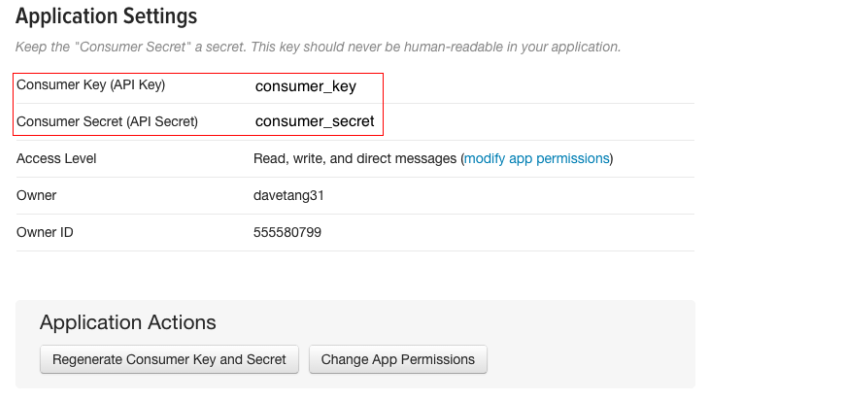
\includegraphics{figures/twitter_app.png}

Setting up the \emph{Twitter OAuth} authentication can be hard, but this
setup should work. We specify the \emph{Consumer Key} and the
\emph{Consumer Secret} and parse it to \emph{setup\_twitter\_oath}.
After this command, the browser will open for authentication. After this
is completed, we can start with submitting our own queries.

\begin{Shaded}
\begin{Highlighting}[]
\KeywordTok{require}\NormalTok{(twitteR)}
\end{Highlighting}
\end{Shaded}

\begin{verbatim}
## Loading required package: twitteR
\end{verbatim}

\begin{Shaded}
\begin{Highlighting}[]
\NormalTok{consumer_key <-}\StringTok{ 'zFnNG5TMJ1jBlUh7ENKjAxTCa'}
\NormalTok{consumer_secret <-}\StringTok{ 'hK6wd2w2zWATEWrmor0brVeSd9jID3YYhmLSnVmj8lp1MErs53'}
\KeywordTok{setup_twitter_oauth}\NormalTok{(consumer_key, consumer_secret)}
\end{Highlighting}
\end{Shaded}

\begin{verbatim}
## [1] "Using browser based authentication"
\end{verbatim}

\section{Constructing the graph of friends and
followers}\label{constructing-the-graph-of-friends-and-followers}

Now we have the connection, we are going to extract some data. For
example, we extract all the tweets from our Chair (the Chair of Systems
Design), whose Twitter Account is \emph{ETHZSystDesign}. We want to
portray the social blueprints of this Twitter account in the first
circle. The friends and followers are retrieved using functions of the
\emph{user} environment of the \emph{TwitteR}-package. Then, we use the
\emph{igraph}-package to draw a graph with this network. A network
consists of

\begin{enumerate}
\def\labelenumi{\arabic{enumi}.}
\itemsep1pt\parskip0pt\parsep0pt
\item
  Nodes (vertices): the Twitter users in the first circle
\item
  Links (edges): directed links exists between vertices and display a
  relation
\end{enumerate}

\begin{itemize}
\itemsep1pt\parskip0pt\parsep0pt
\item
  if $i$ is a follower of $j$, there is a link from $i$ to $j$
\item
  if $i$ is a friends of $j$, there is a link from $j$ to $i$.
\end{itemize}

Please note the syntax of the network: 1. A node
\href{mailto:_@Username}{\_@Username}\_ is added by \emph{network
\textless{}- network + \href{mailto:'@Username'}{'@Username'}} 2. An
edge from $i$ to $j$ is are added by \emph{network{[}i,j{]} \textless{}-
weight}. Instead of $i$ and $j$ one can also use their username
\href{mailto:_'@Username'}{\_'@Username'}\_

First we add all the followers, and after that, we add the friends. A
friend, however, can also be a followers, so we should check whether a
friend already exists as a follower, in order to prevent duplicate
nodes. We to this by constructing a boolean vector with all the nodes
(\emph{V(network)}, V for vertices). If the user already exists, this
vector yields a \emph{TRUE} somewhere. For non-existing users, the
vector only contains \emph{FALSE}. So if the sum of this vector is
\emph{TRUE}, the user is existing and should not be added. If the sum of
this vector yields as \emph{FALSE} the user is non-existing and should
be added. Note that we add a column in the \emph{V(network)}-dataframe
called \emph{\$color}. We assign

\begin{itemize}
\itemsep1pt\parskip0pt\parsep0pt
\item
  for ourself (\href{mailto:_@ETHZSystDesign}{\_@ETHZSystDesign}):
  purple
\item
  followers: yellow
\item
  only friends: red
\item
  both friends and followers: green
\end{itemize}

For the friends, a link is created from
\href{mailto:_@ETHZSystDesign}{\_@ETHZSystDesign}\_ to that friend. For
follower, a link is create from that follower to
\href{mailto:_@ETHZSystDesign_}{\_@ETHZSystDesign\_}. Finally, we plot
the graph with a layout. In this layout, values can take a constant, but
also a different value for every node such as the colour. Then, the
graph is saved in a \emph{.gml}-graph format file. The file is saved in
the working directory of \emph{Rstudio}, one can check the working
directory by typing \emph{getwd()} and set the working directory by
typing \emph{setwd(`your/directory/')}.

\begin{Shaded}
\begin{Highlighting}[]
\KeywordTok{require}\NormalTok{(igraph) }
\NormalTok{user <-}\StringTok{ }\KeywordTok{getUser}\NormalTok{(}\StringTok{'ETHZSystDesign'}\NormalTok{)}
\NormalTok{friends <-}\StringTok{ }\NormalTok{user$}\KeywordTok{getFriends}\NormalTok{()}
\NormalTok{followers <-}\StringTok{ }\NormalTok{user$}\KeywordTok{getFollowers}\NormalTok{()}
\NormalTok{network <-}\KeywordTok{graph.empty}\NormalTok{(}\DataTypeTok{n=}\DecValTok{0}\NormalTok{, }\DataTypeTok{directed=}\OtherTok{TRUE}\NormalTok{)}
\NormalTok{network <-}\StringTok{ }\NormalTok{network +}\StringTok{ }\NormalTok{user$screenName}
\KeywordTok{V}\NormalTok{(network)[user$screenName]$color <-}\StringTok{ 'purple'}
\NormalTok{for (i in }\DecValTok{1}\NormalTok{:}\KeywordTok{length}\NormalTok{(followers))\{}
\NormalTok{network <-}\StringTok{ }\NormalTok{network +followers[[i]]$screenName}
\NormalTok{network[i}\DecValTok{+1}\NormalTok{,}\DecValTok{1}\NormalTok{]<-}\DecValTok{1}
\KeywordTok{V}\NormalTok{(network)[i}\DecValTok{+1}\NormalTok{]$color <-}\StringTok{ 'yellow'}
  \NormalTok{\}}
\NormalTok{for (i in }\DecValTok{1}\NormalTok{:}\KeywordTok{length}\NormalTok{(friends))\{}
  \NormalTok{if (}\KeywordTok{sum}\NormalTok{(}\KeywordTok{V}\NormalTok{(network)$name==friends[[i]]$screenName))\{}
    \NormalTok{network[user$screenName,friends[[i]]$screenName] <-}\StringTok{ }\DecValTok{1}
    \KeywordTok{V}\NormalTok{(network)[friends[[i]]$screenName]$color <-}\StringTok{ 'green'}
    \NormalTok{\}else\{}
      \NormalTok{network <-}\StringTok{ }\NormalTok{network +}\StringTok{ }\NormalTok{friends[[i]]$screenName}
      \NormalTok{network[user$screenName,friends[[i]]$screenName] <-}\StringTok{ }\DecValTok{1}
      \KeywordTok{V}\NormalTok{(network)[friends[[i]]$screenName]$color <-}\StringTok{ 'red'}
    \NormalTok{\}}
\NormalTok{\}}

\KeywordTok{plot}\NormalTok{(network,}
     \DataTypeTok{layout=}\NormalTok{layout.fruchterman.reingold,}
     \DataTypeTok{vertex.size=}\DecValTok{3}\NormalTok{,}
     \DataTypeTok{vertex.color=}\KeywordTok{V}\NormalTok{(network)$color,}
     \DataTypeTok{vertex.label.cex=}\NormalTok{.}\DecValTok{4}\NormalTok{,}
     \DataTypeTok{vertex.label.dist=}\NormalTok{.}\DecValTok{1}\NormalTok{,}
     \DataTypeTok{edge.width =} \FloatTok{0.3}\NormalTok{,}
     \DataTypeTok{edge.arrow.width=}\FloatTok{0.2}\NormalTok{,}
     \DataTypeTok{edge.arrow.size=}\FloatTok{0.4}
     \NormalTok{)}
\end{Highlighting}
\end{Shaded}

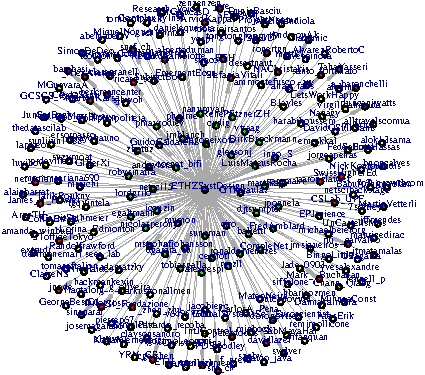
\includegraphics{ETH_Twitter_files/figure-latex/unnamed-chunk-2-1.pdf}

\begin{Shaded}
\begin{Highlighting}[]
\KeywordTok{write.graph}\NormalTok{(network,}\StringTok{"network.gml"}\NormalTok{,}\DataTypeTok{format=}\StringTok{"gml"}\NormalTok{)}
\end{Highlighting}
\end{Shaded}

\section{Save a chunk of tweets into a
\emph{.csv}-file}\label{save-a-chunk-of-tweets-into-a-.csv-file}

A timeline is the set of tweets one user on Twitter has tweeted. This is
an example of a timeline.

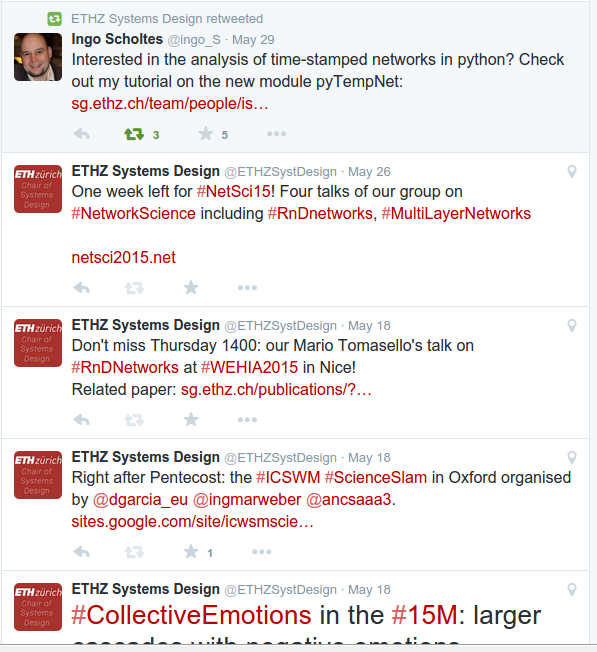
\includegraphics{figures/timeline.png}

Retrieving the timeline can be easily done by using the
\emph{userTimeline} function of the \emph{TwitteR}-package. We take a
big chunk of the timeline, by getting the latest 2000 Tweets (including
retweets). By the time writing, our account has less than 500 tweets so
the function will return all existing tweets. First, we want to save
these tweets in a nice format. Since every tweet has some properties,
the \emph{.csv}-format comes in handy. To write as \emph{.csv} in R, the
least cumbersome way is to convert the tweets intoo a \emph{data.frame}:
the format that R handles very well.

\begin{Shaded}
\begin{Highlighting}[]
\NormalTok{mytweets <-}\KeywordTok{userTimeline}\NormalTok{(user$screenName,}\DataTypeTok{n=}\DecValTok{500}\NormalTok{,}\DataTypeTok{includeRts=}\OtherTok{TRUE}\NormalTok{)}
\NormalTok{df_tweets <-}\KeywordTok{do.call}\NormalTok{(}\StringTok{"rbind"}\NormalTok{,}\KeywordTok{lapply}\NormalTok{(mytweets,as.data.frame))}
\KeywordTok{write.csv}\NormalTok{(df_tweets,}\DataTypeTok{file=}\StringTok{"mytweets.csv"}\NormalTok{)}
\NormalTok{df_tweets[}\DecValTok{1}\NormalTok{:}\DecValTok{3}\NormalTok{,]}
\end{Highlighting}
\end{Shaded}

\begin{verbatim}
##                                                                                                                                       text
## 1  @FETFoCAS covered our latest research on #TemporalNetworks, #ComplexNetworks in which ordering matters.\nhttp://t.co/HL9ms3JfBZ @ingo_S
## 2 @FETFoCAS magazine covered our latest research on #TemporalNetworks : network in which the order matters. @ingo_S http://t.co/HL9ms3JfBZ
## 3                                 Tomorrow at #IFKAD Conference in Bari, Italy, two talks on #RnDNetworks by our Mario Vincenzo Tomasello.
##   favorited favoriteCount replyToSN             created truncated
## 1     FALSE             0  FETFoCAS 2015-06-25 16:53:24     FALSE
## 2     FALSE             0  FETFoCAS 2015-06-22 14:44:51     FALSE
## 3     FALSE             0      <NA> 2015-06-10 10:48:20     FALSE
##   replyToSID                 id replyToUID
## 1         NA 614114179549667328  861230886
## 2         NA 612994663788740608  861230886
## 3         NA 608586489702813696       <NA>
##                                                         statusSource
## 1 <a href="http://twitter.com" rel="nofollow">Twitter Web Client</a>
## 2 <a href="http://twitter.com" rel="nofollow">Twitter Web Client</a>
## 3 <a href="http://twitter.com" rel="nofollow">Twitter Web Client</a>
##       screenName retweetCount isRetweet retweeted longitude latitude
## 1 ETHZSystDesign            0     FALSE     FALSE        NA       NA
## 2 ETHZSystDesign            0     FALSE     FALSE        NA       NA
## 3 ETHZSystDesign            0     FALSE     FALSE        NA       NA
\end{verbatim}

\section{Constructing the graph of Twitter users that mentions
eachother}\label{constructing-the-graph-of-twitter-users-that-mentions-eachother}

In every tweet, it is possible to mention other Twitter user by
including the \_@\_ that indicates a Twitter username.


\includegraphics{figures/tweet.png}

For example, in the above tweet, the name of Twitter user
\href{mailto:_@dgarcia}{\_@dgarcia}\_eu\_,
\href{mailto:_@ingmarweber}{\_@ingmarweber}\_ and
\href{mailto:_@ancsaaa3}{\_@ancsaaa3}\_ are mentioned, probably because
they relate to the tweet.

Rather than the network of friends and followers, we now want to
construct a network of Twitter users who actively interact with
eachother by including eachother username in a tweet.

We should search every tweet for words that start with \emph{@\_ and
ends with a space. Besides that, also usernames in parentheses and
brackets should be extracted. Firstly, we apply the }strsplit\_
function, to split look for spaces, newlines and colons so that we have
a vector with words.

\begin{Shaded}
\begin{Highlighting}[]
\NormalTok{mytweets[}\DecValTok{87}\NormalTok{][[}\DecValTok{1}\NormalTok{]]$text}
\end{Highlighting}
\end{Shaded}

\begin{verbatim}
## [1] "WSBM community detection model succesfully predicts future edges and their weights! @aaronclauset\nhttp://t.co/q1gMqP1aHf"
\end{verbatim}

\begin{Shaded}
\begin{Highlighting}[]
\NormalTok{unlisted_tweet <-}\StringTok{ }\KeywordTok{unlist}\NormalTok{(}\KeywordTok{strsplit}\NormalTok{(mytweets[}\DecValTok{87}\NormalTok{][[}\DecValTok{1}\NormalTok{]]$text, }\StringTok{"}\CharTok{\textbackslash{}n}\StringTok{"}\NormalTok{))}
\NormalTok{unlisted_tweet <-}\StringTok{ }\KeywordTok{unlist}\NormalTok{(}\KeywordTok{strsplit}\NormalTok{(unlisted_tweet, }\StringTok{" "}\NormalTok{))}
\NormalTok{unlisted_tweet <-}\StringTok{ }\KeywordTok{unlist}\NormalTok{(}\KeywordTok{strsplit}\NormalTok{(unlisted_tweet, }\StringTok{":"}\NormalTok{))}
\NormalTok{unlisted_tweet}
\end{Highlighting}
\end{Shaded}

\begin{verbatim}
##  [1] "WSBM"              "community"         "detection"        
##  [4] "model"             "succesfully"       "predicts"         
##  [7] "future"            "edges"             "and"              
## [10] "their"             "weights!"          "@aaronclauset"    
## [13] "http"              "//t.co/q1gMqP1aHf"
\end{verbatim}

we use the \emph{grep} function to extract every word that starts with
\emph{@\_ or with brackets or parentheses, followed by }@\_. Then, we
use the \emph{gsub} function to strip all the alphanumeric character
(such as brackets, parentheses and comma's). We bind the result in a
\emph{data.frame} so that we have every instance of our account
\emph{ETHZSystDesign} mentioning another Twitter user.

\begin{Shaded}
\begin{Highlighting}[]
\NormalTok{extract_users <-}\StringTok{ }\NormalTok{function(mytweets)\{}
\NormalTok{mentions <-}\KeywordTok{data.frame}\NormalTok{(}\DataTypeTok{createdName=}\KeywordTok{character}\NormalTok{(),}
                      \DataTypeTok{quotedName=}\KeywordTok{character}\NormalTok{(),}
                      \DataTypeTok{stringsAsFactors=}\OtherTok{FALSE}\NormalTok{)}
\NormalTok{for (i in }\DecValTok{1}\NormalTok{:}\KeywordTok{length}\NormalTok{(mytweets))\{}
  \NormalTok{name_indices <-}\StringTok{ }\KeywordTok{gregexpr}\NormalTok{(}\DataTypeTok{pattern=}\StringTok{"@"}\NormalTok{,mytweets[[i]]$text)}
  \NormalTok{unlisted_tweet <-}\StringTok{ }\KeywordTok{unlist}\NormalTok{(}\KeywordTok{strsplit}\NormalTok{(mytweets[i][[}\DecValTok{1}\NormalTok{]]$text, }\StringTok{"}\CharTok{\textbackslash{}n}\StringTok{"}\NormalTok{))}
  \NormalTok{unlisted_tweet <-}\StringTok{ }\KeywordTok{unlist}\NormalTok{(}\KeywordTok{strsplit}\NormalTok{(unlisted_tweet, }\StringTok{" "}\NormalTok{))}
  \NormalTok{unlisted_tweet <-}\StringTok{ }\KeywordTok{unlist}\NormalTok{(}\KeywordTok{strsplit}\NormalTok{(unlisted_tweet, }\StringTok{":"}\NormalTok{))}
  \NormalTok{regex1 <-}\StringTok{ "(^|[^@}\CharTok{\textbackslash{}\textbackslash{}}\StringTok{w])@(}\CharTok{\textbackslash{}\textbackslash{}}\StringTok{w\{1,15\})}\CharTok{\textbackslash{}\textbackslash{}}\StringTok{b"} \CommentTok{# get strings with @}
\NormalTok{regex2 <-}\StringTok{ "[^[:alnum:]@_]"}             \CommentTok{# remove all punctuation except _ and @}
\NormalTok{users <-}\StringTok{ }\KeywordTok{gsub}\NormalTok{(regex2, }\StringTok{""}\NormalTok{, unlisted_tweet[}\KeywordTok{grep}\NormalTok{(regex1, unlisted_tweet, }\DataTypeTok{perl =} \NormalTok{T)])}
\NormalTok{mentions <-}\StringTok{ }\KeywordTok{rbind}\NormalTok{(mentions,}\KeywordTok{data.frame}\NormalTok{(}\KeywordTok{rep}\NormalTok{(}\KeywordTok{paste}\NormalTok{(}\StringTok{"@"}\NormalTok{,mytweets[i][[}\DecValTok{1}\NormalTok{]]$screenName,}\DataTypeTok{sep=}\StringTok{""}\NormalTok{),}\KeywordTok{length}\NormalTok{(users)),users, }\DataTypeTok{stringsAsFactors=}\OtherTok{FALSE}\NormalTok{))}
\NormalTok{\}  }
\KeywordTok{colnames}\NormalTok{(mentions) <-}\StringTok{ }\KeywordTok{c}\NormalTok{(}\StringTok{"createdName"}\NormalTok{,}\StringTok{"quotedName"}\NormalTok{)}
\KeywordTok{return}\NormalTok{(mentions)}
\NormalTok{\}}
\NormalTok{mentions <-}\StringTok{ }\KeywordTok{extract_users}\NormalTok{(mytweets)}
\NormalTok{mentions[}\DecValTok{1}\NormalTok{:}\DecValTok{5}\NormalTok{,]}
\end{Highlighting}
\end{Shaded}

\begin{verbatim}
##       createdName quotedName
## 1 @ETHZSystDesign  @FETFoCAS
## 2 @ETHZSystDesign    @ingo_S
## 3 @ETHZSystDesign  @FETFoCAS
## 4 @ETHZSystDesign    @ingo_S
## 5 @ETHZSystDesign    @ingo_S
\end{verbatim}

We now need frequency counts of username to achieve the number of
mentions. We use the table function and create another network. For
every mention, we create a link between
\href{mailto:_@ETHZSystDesign}{\_@ETHZSystDesign}\_ and the
corresponding user. We also assign a link weight with the corresponding
times of being mentioned. We make this visible in the plot, by giving
every link a variable \emph{edge.width}, given by the weights.

\begin{Shaded}
\begin{Highlighting}[]
\NormalTok{mentions_tab <-}\StringTok{ }\KeywordTok{table}\NormalTok{(mentions$quotedName)}
\NormalTok{network <-}\KeywordTok{graph.empty}\NormalTok{(}\DataTypeTok{n=}\DecValTok{0}\NormalTok{, }\DataTypeTok{directed=}\OtherTok{TRUE}\NormalTok{)}
\NormalTok{network <-}\StringTok{ }\NormalTok{network +}\StringTok{ }\NormalTok{user$screenName}
\KeywordTok{V}\NormalTok{(network)[user$screenName]$color <-}\StringTok{ 'purple'}
\NormalTok{for (i in }\DecValTok{1}\NormalTok{:}\KeywordTok{nrow}\NormalTok{(mentions_tab))\{}
  \NormalTok{network <-}\StringTok{ }\NormalTok{network +}\StringTok{ }\KeywordTok{rownames}\NormalTok{(mentions_tab)[i]}
  \NormalTok{network[user$screenName, }\KeywordTok{rownames}\NormalTok{(mentions_tab)[i]] <-}\StringTok{ }\DecValTok{1}
  \KeywordTok{E}\NormalTok{(network)[i]$weight <-}\StringTok{ }\NormalTok{mentions_tab[i] }
\NormalTok{\}}
\KeywordTok{plot}\NormalTok{(network,}
     \DataTypeTok{layout=}\NormalTok{layout.fruchterman.reingold,}
     \DataTypeTok{vertex.size=}\DecValTok{3}\NormalTok{,}
     \DataTypeTok{vertex.label.cex=}\NormalTok{.}\DecValTok{4}\NormalTok{,}
     \DataTypeTok{vertex.label.dist=}\NormalTok{.}\DecValTok{2}\NormalTok{,}
     \DataTypeTok{edge.width =} \KeywordTok{E}\NormalTok{(network)$weight, }
     \DataTypeTok{edge.arrow.width=}\NormalTok{.}\DecValTok{5}
     \NormalTok{)}
\end{Highlighting}
\end{Shaded}

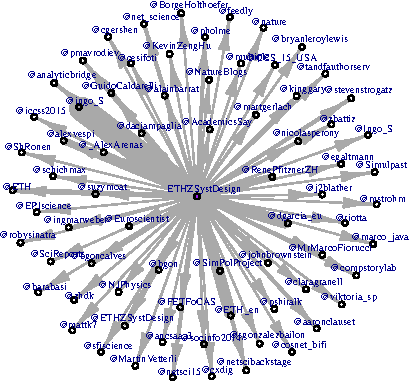
\includegraphics{ETH_Twitter_files/figure-latex/unnamed-chunk-6-1.pdf}
\# Construct the network of quoting users with a certain hashtag We have
constructed network from the perspective of one user: one user was
portrayed in the middle and his friends, followers and tweets were
investigated. We know are going to apply a real-world scenario. We will
scrape the Twitter universe for a certain hashtag and see which people
mention eachother.

We will reuse the function \emph{extract\_user}, which we used earlier
on already. A hashtag is specified and we will again have a \emph{names}
dataframe containing in a mention-link from column 1 to column 2. Again,
we constructed an \emph{igraph}-network.

\subsection{Preventing adding same users
twice}\label{preventing-adding-same-users-twice}

Every user that does not exist in the network, should be added manually.
The \emph{add\_if\_not\_exits} function checks the complete vertex
sequence and checks if the current name is in that sequence. If the user
is not in the vertex sequence, it outputs a vector containing only
\emph{FALSE} elements. If the user already exists, one elements will be
\emph{TRUE} so it's sum will also be true. A exclamation mark is added,
so that if the sum is \emph{FALSE} (e.g.~the user does not exists yet),
the user is added afterwards.

\subsection{Constructing and plotting}\label{constructing-and-plotting}

We use \emph{igraph} again for adding the edges and plotting the graph.

\begin{Shaded}
\begin{Highlighting}[]
\NormalTok{add_if_not_exists <-}\StringTok{ }\NormalTok{function(network,name)\{}
    \NormalTok{if (!}\KeywordTok{sum}\NormalTok{(}\KeywordTok{V}\NormalTok{(network)$name==name)) \{}
    \NormalTok{network <-}\StringTok{ }\NormalTok{network +}\StringTok{ }\NormalTok{name \}}
  \KeywordTok{return}\NormalTok{(network)}
\NormalTok{\}}
\NormalTok{hashtag <-}\StringTok{ '#itsacoup'}
\NormalTok{hashsearch <-}\StringTok{ }\KeywordTok{searchTwitter}\NormalTok{(hashtag,}\DataTypeTok{n=}\DecValTok{100}\NormalTok{)}
\NormalTok{names <-}\StringTok{ }\KeywordTok{extract_users}\NormalTok{(hashsearch)}
\NormalTok{network <-}\KeywordTok{graph.empty}\NormalTok{(}\DataTypeTok{n=}\DecValTok{0}\NormalTok{, }\DataTypeTok{directed=}\OtherTok{TRUE}\NormalTok{)}
\NormalTok{for (i in }\DecValTok{1}\NormalTok{:}\KeywordTok{nrow}\NormalTok{(names))\{}
  \NormalTok{network <-}\StringTok{ }\KeywordTok{add_if_not_exists}\NormalTok{(network,names[i,}\DecValTok{1}\NormalTok{])}
  \NormalTok{network <-}\StringTok{ }\KeywordTok{add_if_not_exists}\NormalTok{(network,names[i,}\DecValTok{2}\NormalTok{])}
  \NormalTok{network <-}\StringTok{ }\KeywordTok{add.edges}\NormalTok{(network,}\KeywordTok{c}\NormalTok{(names[i,}\DecValTok{1}\NormalTok{],names[i,}\DecValTok{2}\NormalTok{]))}
  \NormalTok{\}}
\KeywordTok{plot}\NormalTok{(network,}
     \DataTypeTok{layout=}\NormalTok{layout.fruchterman.reingold,}
     \DataTypeTok{vertex.size=}\DecValTok{4}\NormalTok{,}
     \DataTypeTok{vertex.label.cex=}\NormalTok{.}\DecValTok{5}\NormalTok{,}
     \DataTypeTok{vertex.label.dist=}\NormalTok{.}\DecValTok{2}\NormalTok{,}
     \DataTypeTok{edge.width =} \NormalTok{.}\DecValTok{5}\NormalTok{,}
     \DataTypeTok{edge.arrow.width=}\NormalTok{.}\DecValTok{3}\NormalTok{,}
     \DataTypeTok{edge.arrow.size=}\NormalTok{.}\DecValTok{5}
     \NormalTok{)}
\end{Highlighting}
\end{Shaded}

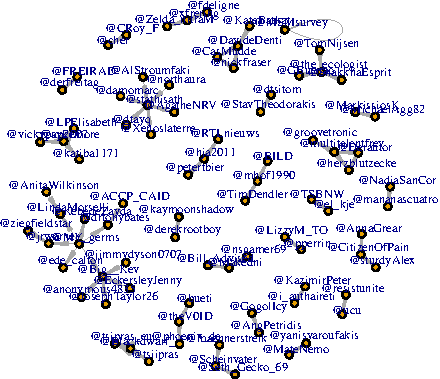
\includegraphics{ETH_Twitter_files/figure-latex/unnamed-chunk-7-1.pdf}

\end{document}
